\documentclass{beamer}

\mode<presentation>
\usetheme{Madrid}

\usepackage[spanish]{babel}
\usepackage[utf8]{inputenc}
\usepackage[T1]{fontenc} % hyphenation 
\usepackage{times}
\usepackage{tikz}
\usepackage{fourier}
\usepackage{gensymb}
\usepackage{amsmath}

\setbeamercovered{dynamic}

\title[Sensores Remotos]{Sensores remotos}
\subtitle[]{Curso de Zonificación Vitícola y Viticultura de Precisión}


\author[G.F. Olmedo]{Guillermo Federico Olmedo}

\institute[INTA] % (optional, but mostly needed)
{ Laboratorio de Geomática\\
  Recursos Naturales\\
  INTA EEA Mendoza\\
  \vskip10pt
\begin{columns}
	\column{.5\textwidth}
	\begin{flushright}
		
\includegraphics[width=1.7cm]{IMGs/logoINTA}
	\end{flushright}
	\column{.5\textwidth}
	\begin{flushleft}
		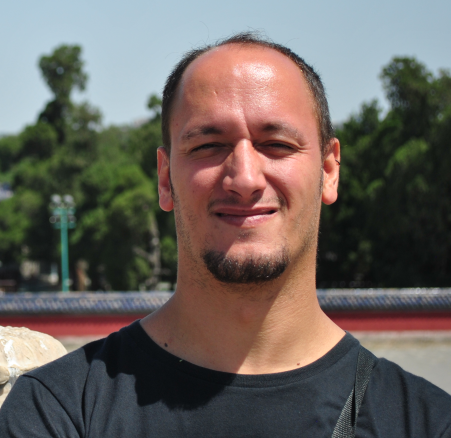
\includegraphics[width=1.7cm]{IMGs/yo}
	\end{flushleft}
\end{columns}  
}

\date[FCA, 16-20/05/2016]{Fac. de Cs. Agrarias, 16 al 20 de mayo de 2016}

\pgfdeclareimage[height=0.5cm]{university-logo}{IMGs/logoINTA}
\logo{\pgfuseimage{university-logo}}

%\beamerdefaultoverlayspecification{<+->}


\begin{document}

\begin{frame}[plain]
  \titlepage
\end{frame}

\begin{frame}{Outline}
	\tableofcontents[pausesections]
	% You might wish to add the option [pausesections]
\end{frame}

\section{Introducción}

\begin{frame}{Principales ventanjas de los sensores satelitales}
	\begin{itemize}
		\item Visión global.
		\item Observación a distintas escalas.
		\item Cobertura frecuente.
		\item Homogeneidad en la adquisición.
		\item Regiones no visibles del espectro.
		\item Formato digital.
	\end{itemize}
\end{frame}

\begin{frame}{Diferentes escalas}
	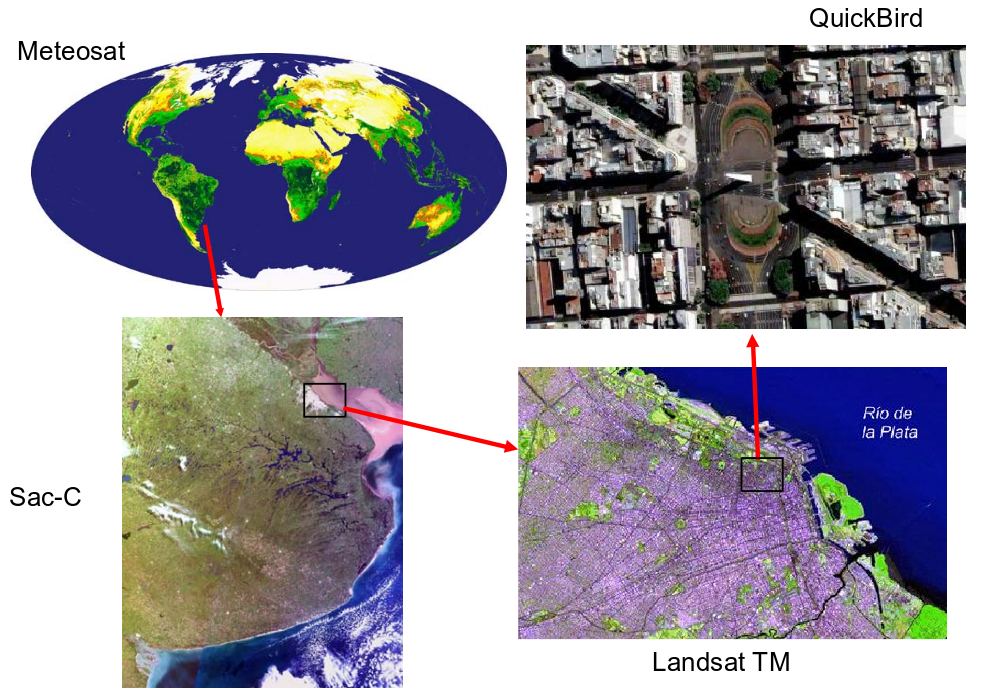
\includegraphics[width=0.95\textwidth]{IMGs/resoluciones}
\end{frame}

\begin{frame}{Homogeneidad en la adquisición}
	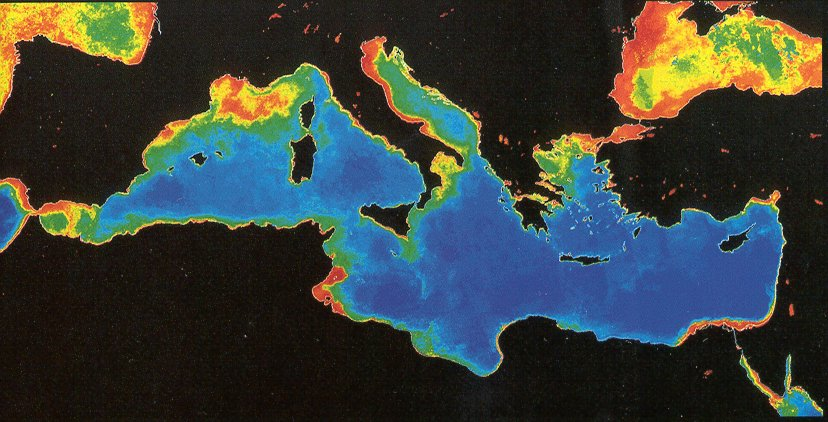
\includegraphics[width=\textwidth]{IMGs/fitop}\footnote{SEAWIFS}
\end{frame}

\begin{frame}{Regiones no visibles}
	\centering
	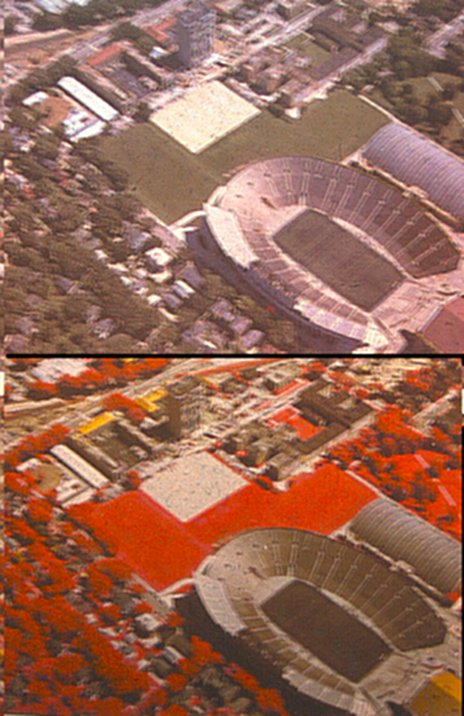
\includegraphics[width=0.4\textwidth]{IMGs/VISNIR}
\end{frame}

\begin{frame}{Inconvenientes}
	\begin{itemize}
		\item Requieren calibración.
		\item Cobertura nubosa.
		\item Frecuencia de adquisición.
		\item Resolución espacial.
		\item Resolución espectral.
	\end{itemize}
\end{frame}

\section{Principios físicos}

\begin{frame}{Tipos de procesos en teledetección}
	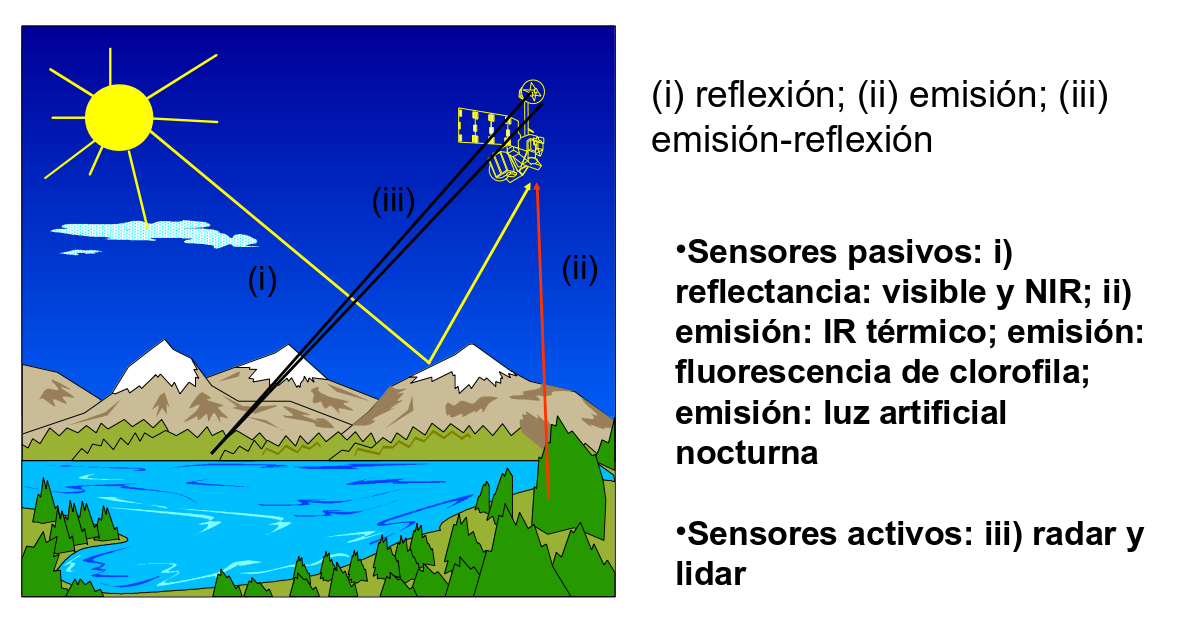
\includegraphics[width=\textwidth]{IMGs/procesos}
\end{frame}

\begin{frame}{Las ondas electromagnéticas}
	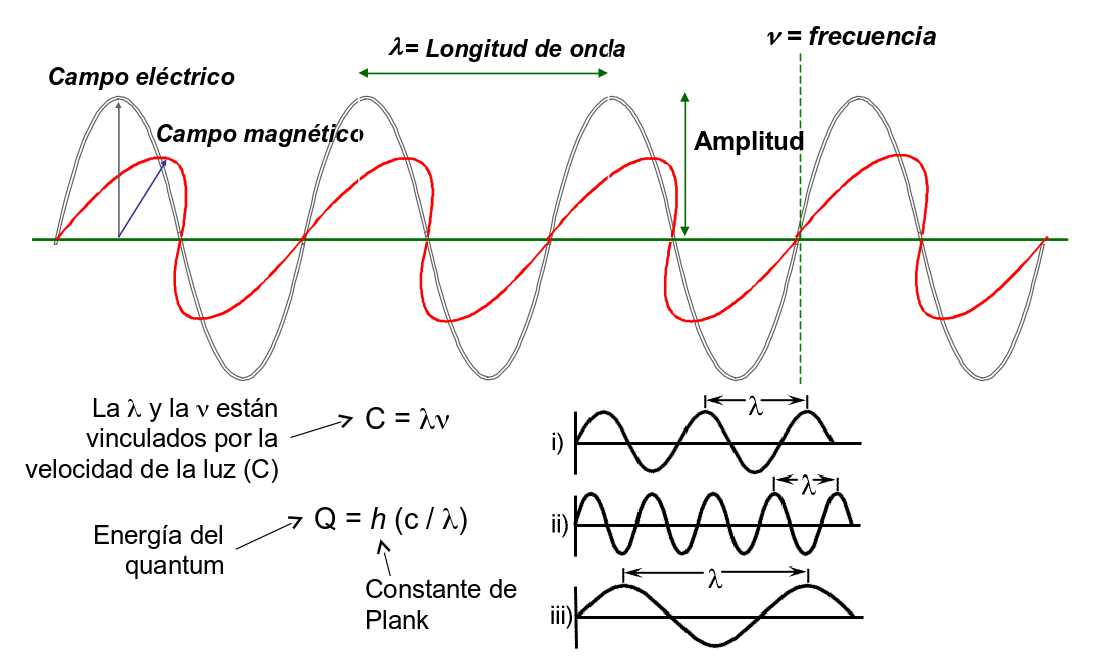
\includegraphics[width=\textwidth]{IMGs/ondas}
\end{frame}

\begin{frame}{El espectro electromagnético}
	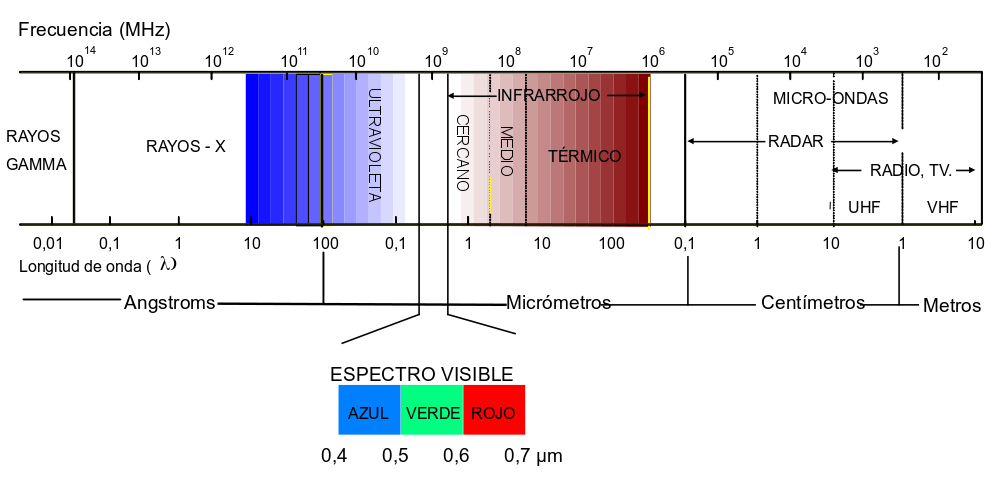
\includegraphics[width=\textwidth]{IMGs/espectro}
\end{frame}

\begin{frame}{Emitancia radiativa del cuerpo negro}
	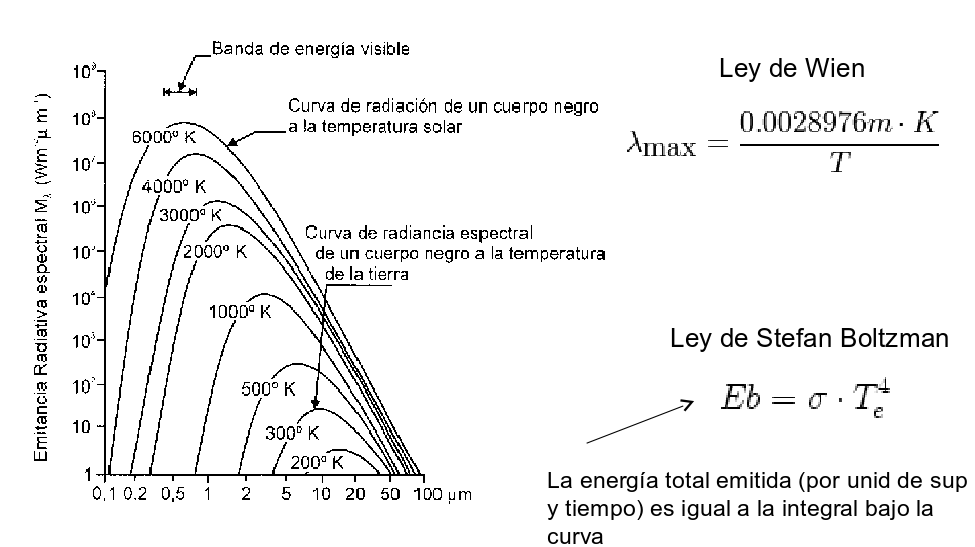
\includegraphics[width=\textwidth]{IMGs/law1}
\end{frame}

\begin{frame}{Emitancia radiativa del sol}
	\centering
	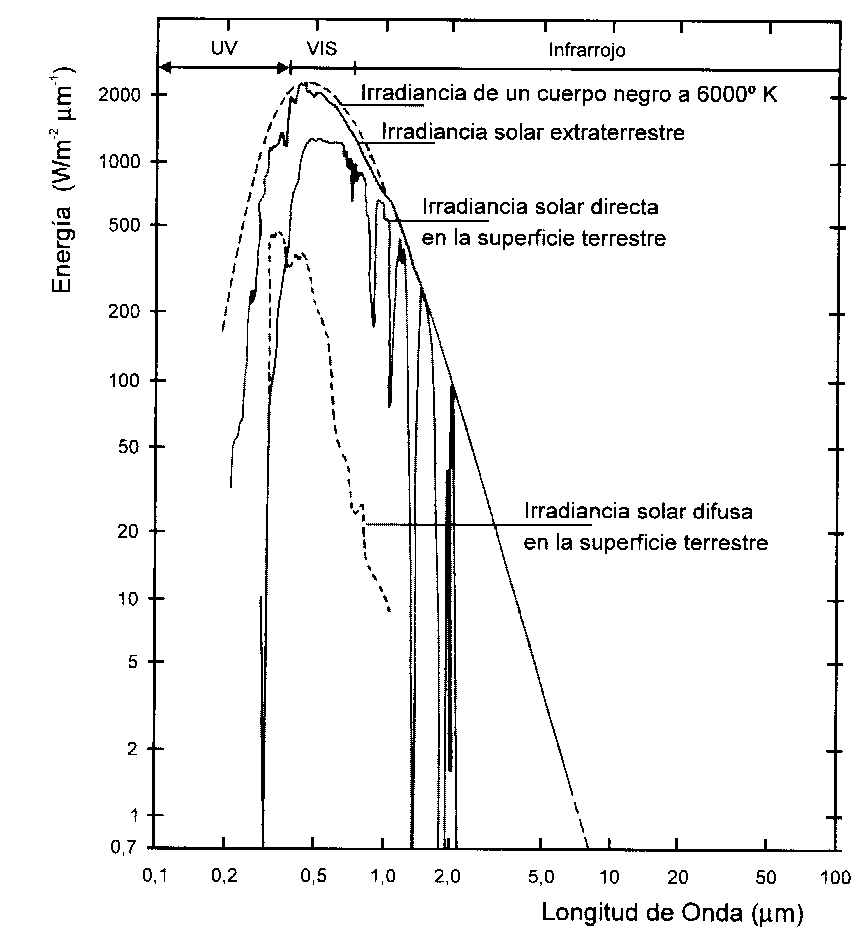
\includegraphics[width=0.6\textwidth]{IMGs/law2}
\end{frame}

\begin{frame}{Dispersión atmosférica}
	\begin{columns}
				\column{.45\textwidth}
				\begin{itemize}
					\item Factores:
					\begin{itemize}
						\item Vapor de agua.
						\item Partículas en suspensión.
					\end{itemize}
					\item Tipos:
					\begin{itemize}
						\item Rayleigh: $\sigma$ < $\lambda$ . Afecta a las más cortas y es la más intensa: cielo.
						\item Mie: $\sigma$ 0 $\lambda$. Afectan a mayores $\lambda$: aerosoles y polvo atmosférico).
						\item No selectiva. $\sigma$ > $\lambda$. Por igual en cualquier $\lambda$: nubes
					\end{itemize}
					
				\end{itemize}
				\column{.45\textwidth}
				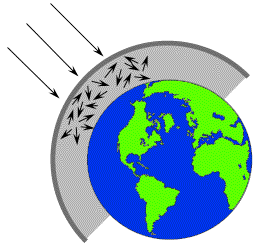
\includegraphics[width=0.5\textwidth]{IMGs/dispersion}\\
				\bigskip
				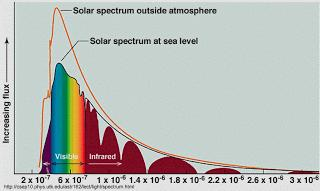
\includegraphics[width=0.7\textwidth]{IMGs/solar_spectrum}
	\end{columns}
\end{frame}

\begin{frame}{El flujo incidente}
	\begin{columns}
		\column{.45\textwidth}
		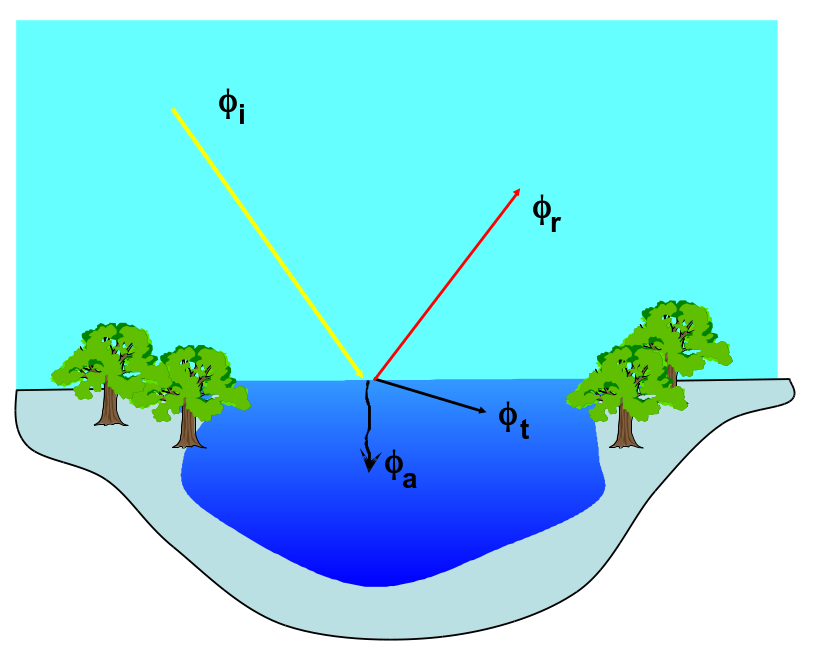
\includegraphics[width=\textwidth]{IMGs/flujo}
		\column{.45\textwidth}
		\begin{align}
		\phi_i & =  \phi_r + \phi_a + \phi_t \notag \\
		\frac{\phi_i}{\phi_i} & =  \frac{\phi_r}{\phi_i} + \frac{\phi_a}{\phi_i} + \frac{\phi_t}{\phi_i} \notag \\
		1 & =  \rho + \alpha + \tau \notag  \\
		1 & =  \rho_\lambda + \alpha_\lambda + \tau_\lambda \notag 
		\end{align}	
	\end{columns}
	\bigskip
	{\footnotesize Donde $\phi_i$ es el flujo incidente, $\phi_r$ es el flujo reflejado, $\phi_a$ es el flujo absorvido y $\phi_t$ es el flujo trasmitido.}
\end{frame}

\begin{frame}{Factores que inciden en la reflexión de las cubiertas}
	\begin{itemize}
		\item Elementos que absorben (agua, pigmentos, minerales).
		\item Rugosidad superficial (reflectividad lambertiana o especular).
		\item Ángulos de observación e iluminación.
	\end{itemize}
\end{frame}

\begin{frame}{Tipos de reflectores}
	\centering
	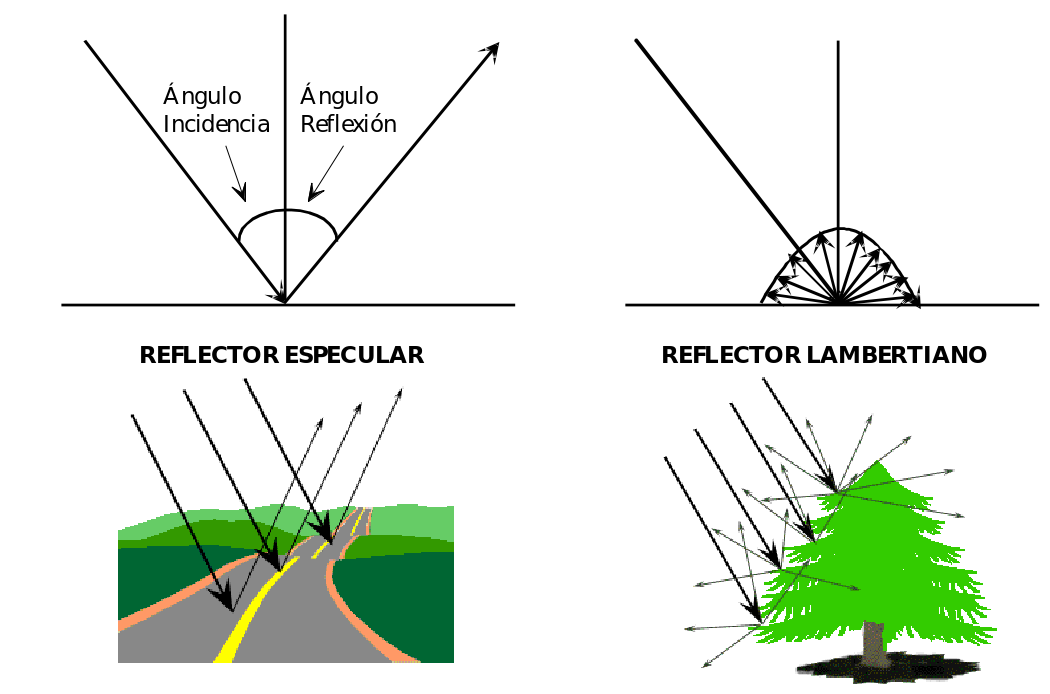
\includegraphics[width=0.8\textwidth]{IMGs/reflectores}
\end{frame}

\section{Reflectancia y vegetación}

\begin{frame}{La reflectancia en la vegetación}
	\begin{itemize}
		\item Factores que dependen de la canopia.
		\begin{itemize}
			\item Proporción hoja / tallos / suelo
			\item Geometría de las hojas.
			\item Ángulos de observación.
		\end{itemize}
		\item Factores que dependen de la hoja.
		\begin{itemize}
			\item Pigmentos.
			\item Estructura de la hoja.
			\item Humedad
		\end{itemize}
	\end{itemize}
\end{frame}

\begin{frame}{Curva característica de una hoja}
	\centering
	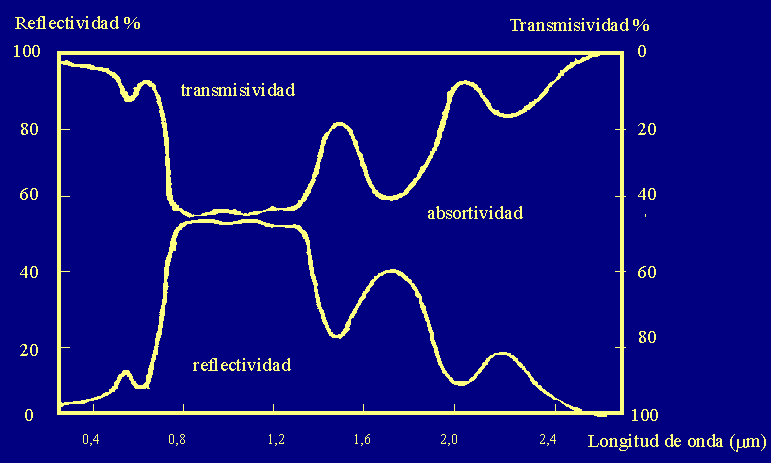
\includegraphics[width=0.9\textwidth]{IMGs/curvahoja}
\end{frame}

\begin{frame}{Reflectividad en la hoja}
	\centering
	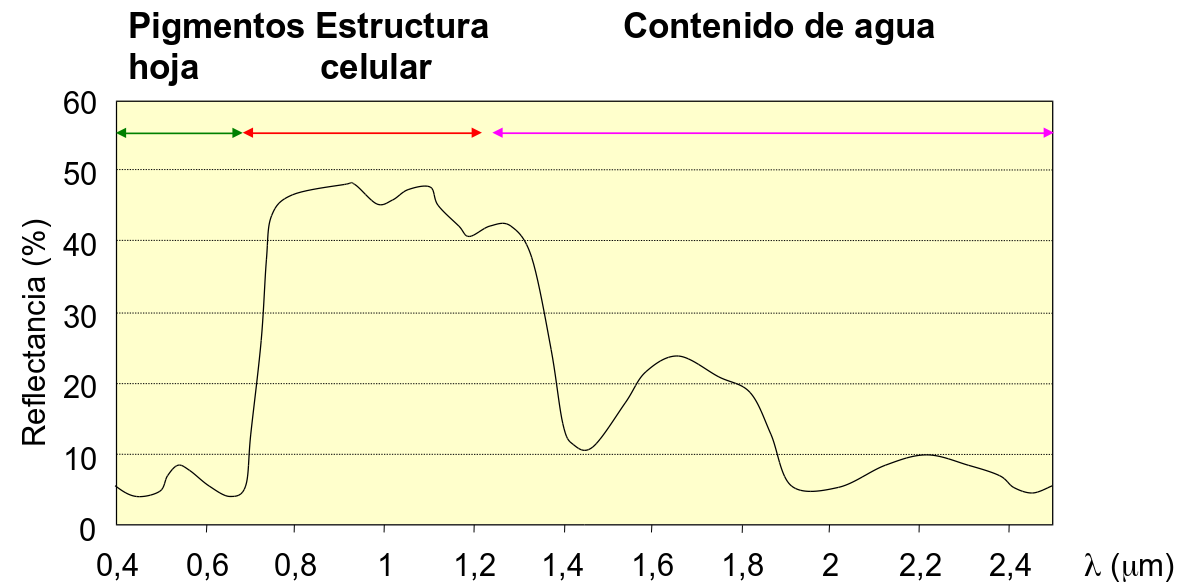
\includegraphics[width=1\textwidth]{IMGs/reflechoja}
\end{frame}

\begin{frame}{Estructura de la hoja y la luz}
	\centering
	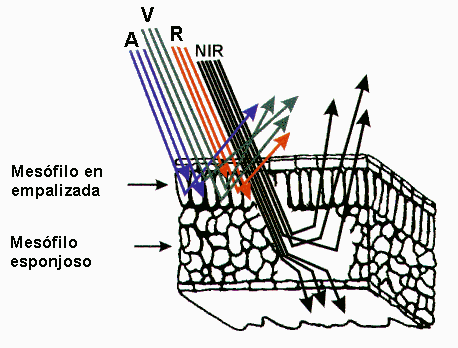
\includegraphics[width=0.8\textwidth]{IMGs/hojayluz}
\end{frame}

\begin{frame}{Firmas espectrales}
	\centering
	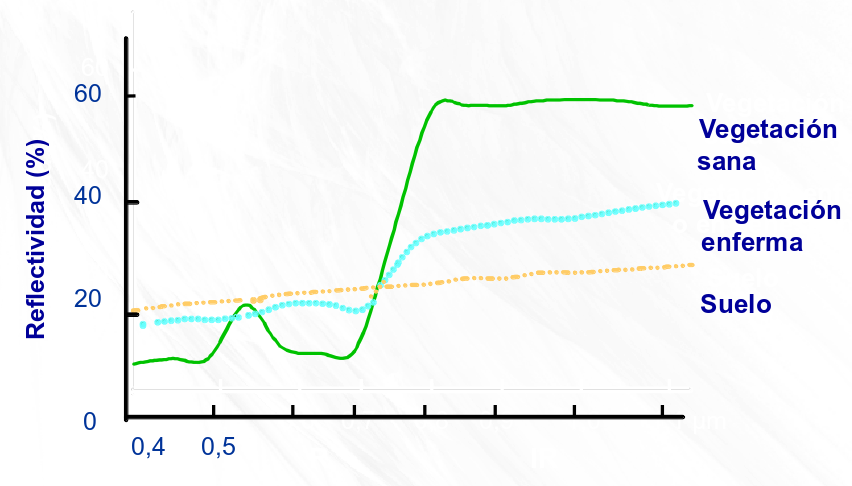
\includegraphics[width=1\textwidth]{IMGs/vegetacion}
\end{frame}

\begin{frame}{Firmas espectrales}
	\begin{columns}
		\column{.45\textwidth}
		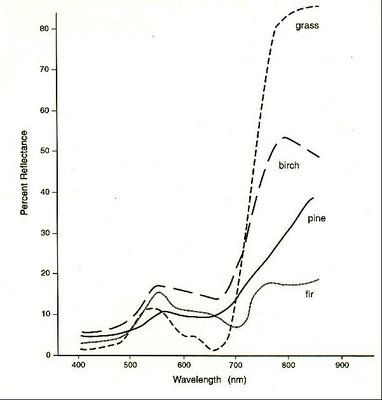
\includegraphics[width=1\textwidth]{IMGs/especies}
		\column{.45\textwidth}
		\includegraphics<2>[width=0.8\textwidth]{IMGs/leafdamage}
	\end{columns}
\end{frame}

\begin{frame}{Arquitectura}
	\begin{columns}
		\column{.45\textwidth}
		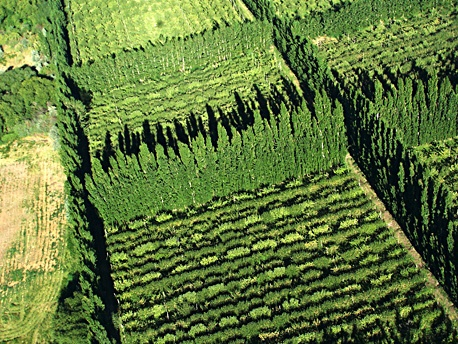
\includegraphics[width=1\textwidth]{IMGs/geometria}
		\column{.45\textwidth}
		\includegraphics<2>[width=1\textwidth]{IMGs/dosel}
	\end{columns}
\end{frame}

\section{Sensores Remotos}

\begin{frame}{Plataformas}
	\begin{columns}
		\column{.35\textwidth}
		\begin{itemize}
			\item Terrestres.
			\item Aéreas.
			\item Espaciales:
			Geo-estacionarios (36.000 km).
			Órbitas bajas (200-1000 km):
			\begin{itemize}
				\item Polar: heliosíncronos.
				\item Ecuatorial.
			\end{itemize}
		\end{itemize}
		\column{.65\textwidth}
		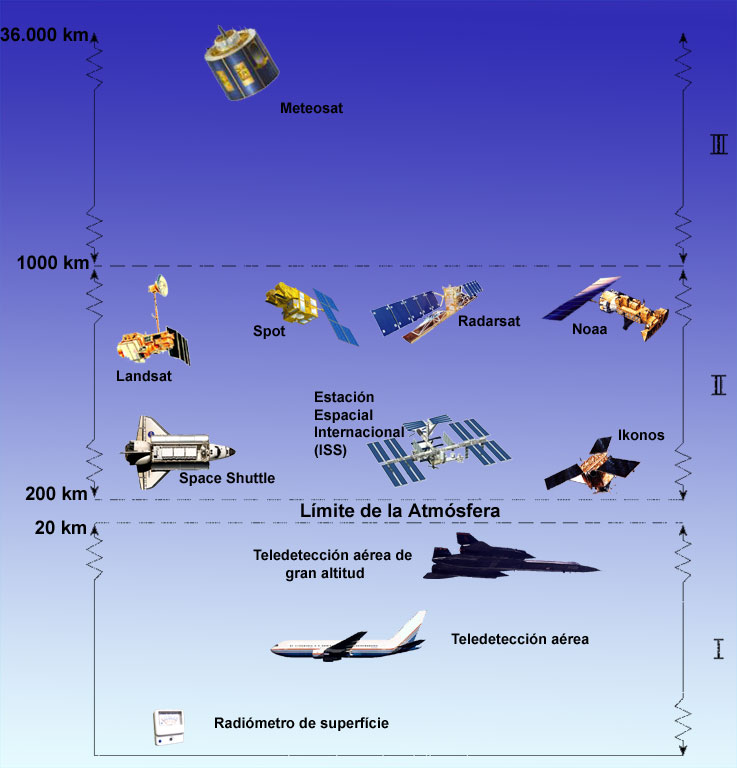
\includegraphics[width=1\textwidth]{IMGs/plataforma}
	\end{columns}
\end{frame}

\begin{frame}{Características de los sensores}{Resoluciones}
	\begin{columns}[t]
		\column{.5\textwidth}
		\begin{itemize}
			\item Espacial \\
			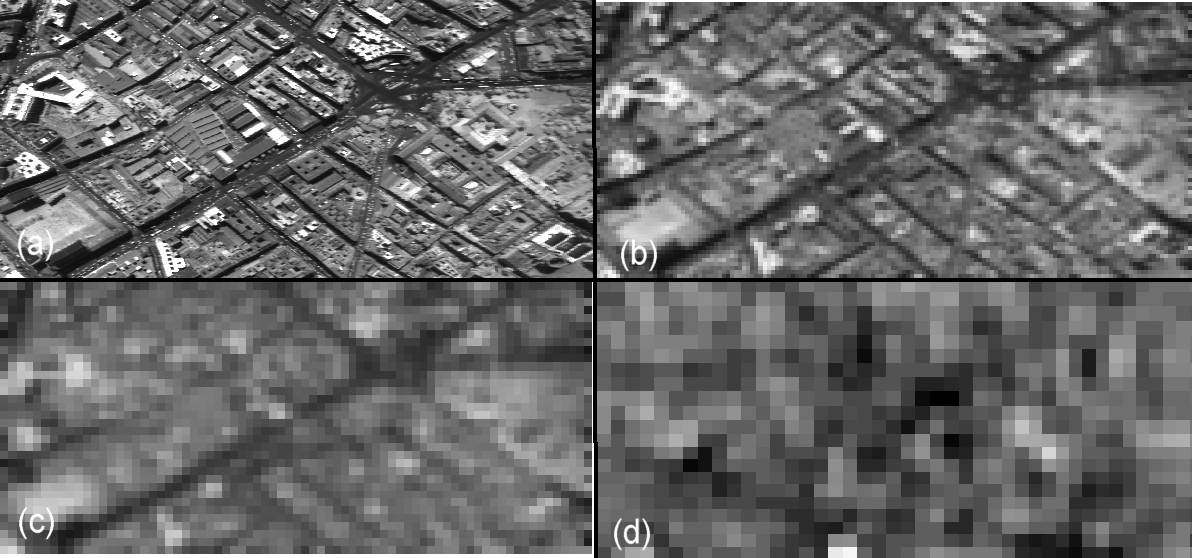
\includegraphics[width=0.8\textwidth]{IMGs/res_esp}
			\item Espectral
			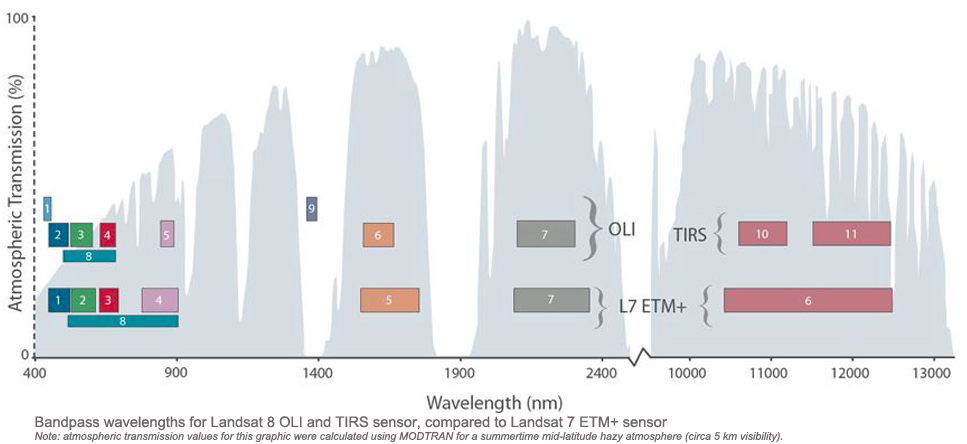
\includegraphics[width=0.8\textwidth]{IMGs/res_spectral}
		\end{itemize}
		\column{.5\textwidth}
		\begin{itemize}

		\item Temporal \\
		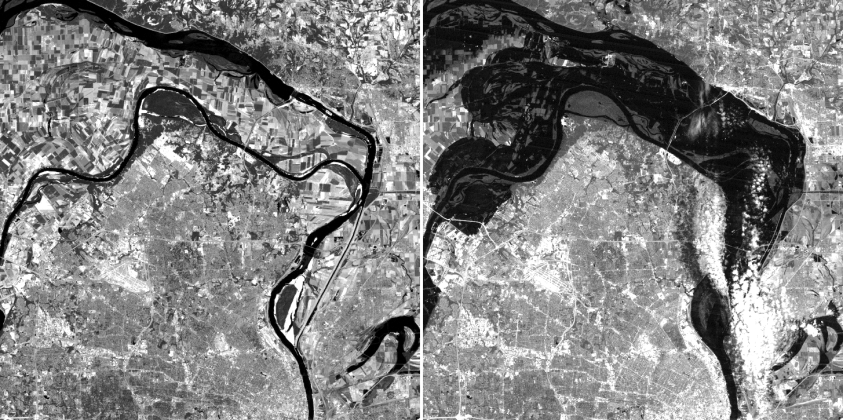
\includegraphics[width=0.8\textwidth]{IMGs/res_temp}
		\item Radiométrica
		\begin{columns}
			\column{.33\textwidth}
			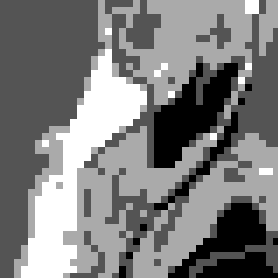
\includegraphics[width=1\textwidth]{IMGs/res_rad2}
			\column{.33\textwidth}
			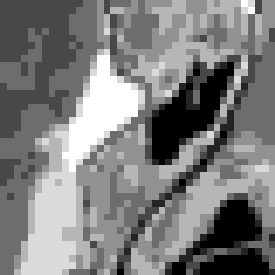
\includegraphics[width=1\textwidth]{IMGs/res_rad3}
			\column{.33\textwidth}
			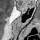
\includegraphics[width=1\textwidth]{IMGs/res_rad4}
		\end{columns}	
		\end{itemize}
	\end{columns}
	Angular \ldots
\end{frame}

\begin{frame}{Resolución Espacial}
	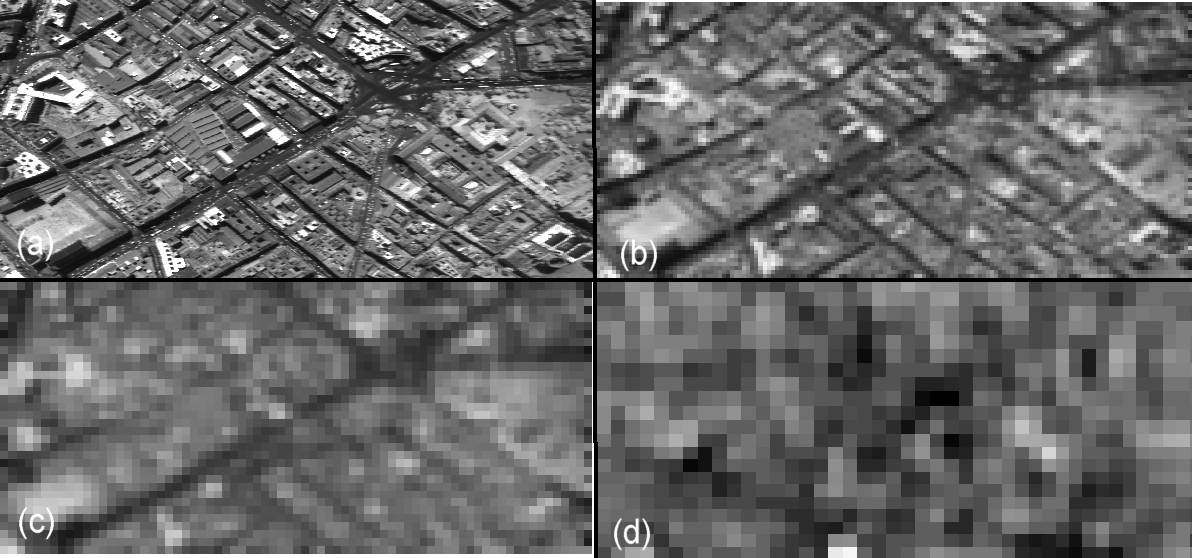
\includegraphics[width=1\textwidth]{IMGs/res_esp}
\end{frame}

\begin{frame}{Resolución Espacial}
	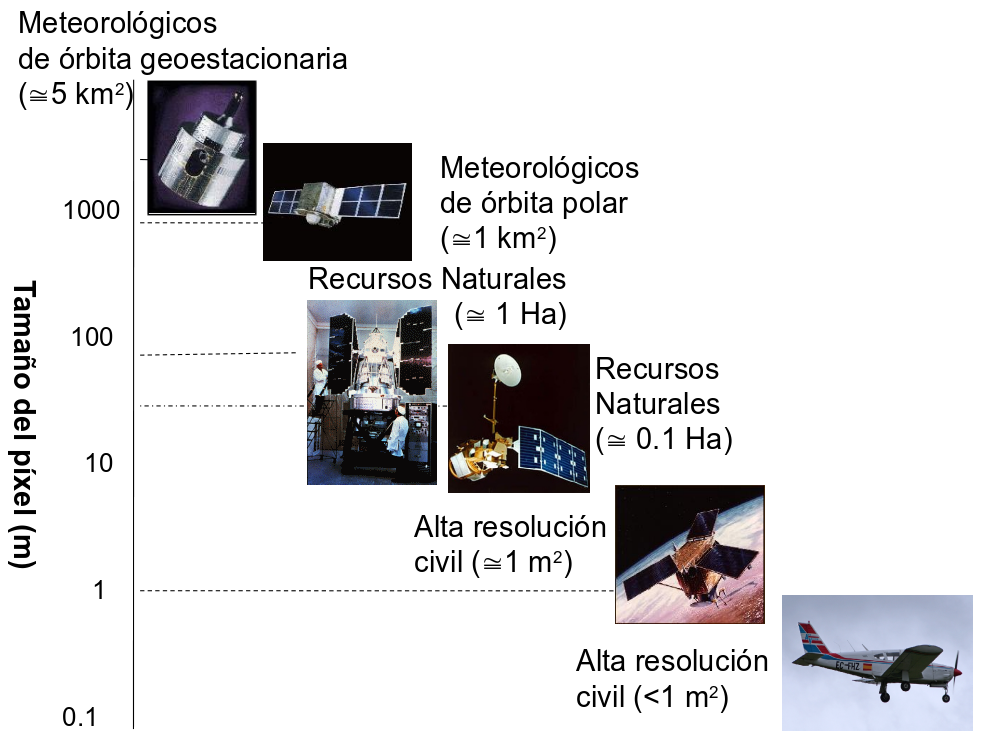
\includegraphics[width=0.9\textwidth]{IMGs/res_espacial2}
\end{frame}

\begin{frame}{Resolución radiométrica}
	\begin{columns}
		\column{.33\textwidth}
		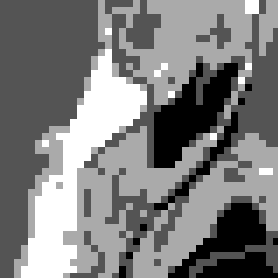
\includegraphics[width=1\textwidth]{IMGs/res_rad2}\\
		2 bits = 4 tonos
		\column{.33\textwidth}
		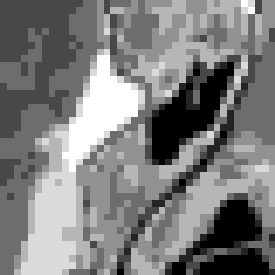
\includegraphics[width=1\textwidth]{IMGs/res_rad3}\\
		3 bits = 8 tonos
		\column{.33\textwidth}
		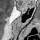
\includegraphics[width=1\textwidth]{IMGs/res_rad4}\\
		4 bits = 16 tonos
	\end{columns}	
\end{frame}

\begin{frame}{Resolución radiométrica}
		\begin{columns}
			\column{.5\textwidth}
			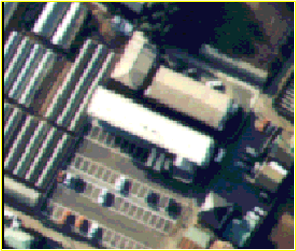
\includegraphics[width=0.65\textwidth]{IMGs/rad_luz1}\\
			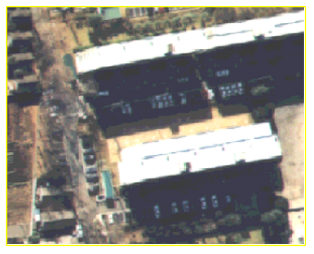
\includegraphics[width=0.65\textwidth]{IMGs/rad_dark1}
			\column{.5\textwidth}
			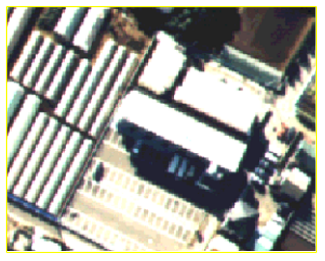
\includegraphics[width=0.65\textwidth]{IMGs/rad_luz2}\\
			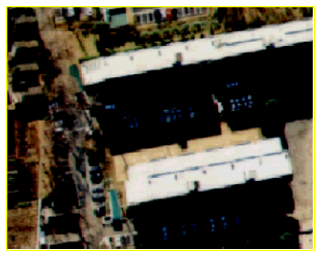
\includegraphics[width=0.65\textwidth]{IMGs/rad_dark2}
		\end{columns}
\end{frame}

\begin{frame}{Resolución Espectral}
	\centering
	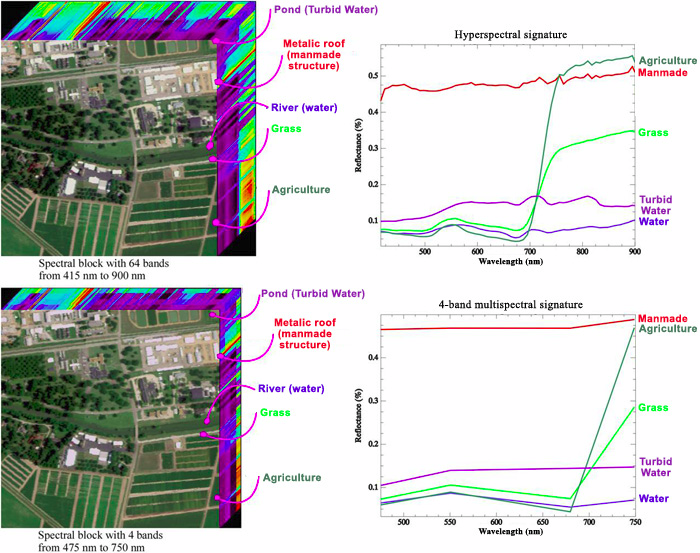
\includegraphics[width=0.8\textwidth]{IMGs/res_spectral2}
\end{frame}

\begin{frame}{Resolución Espectral}
	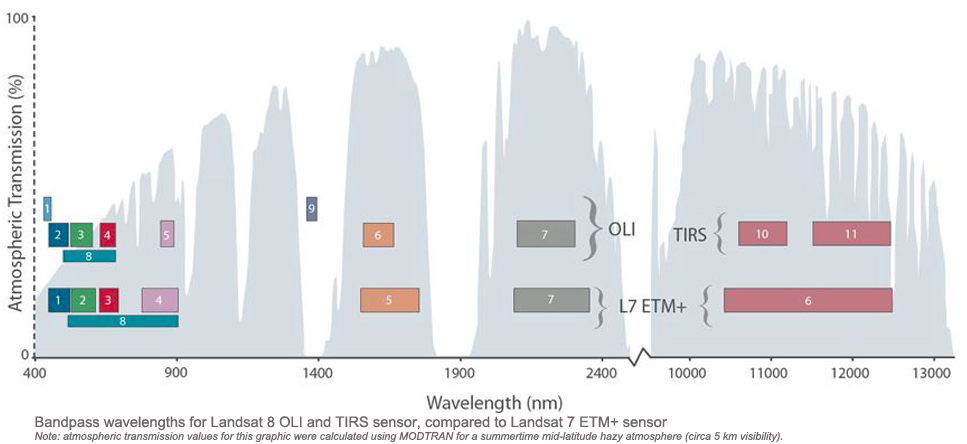
\includegraphics[width=1\textwidth]{IMGs/res_spectral}
\end{frame}

\begin{frame}{Cámaras multiespectrales}
	\begin{columns}
		\column{.5\textwidth}
		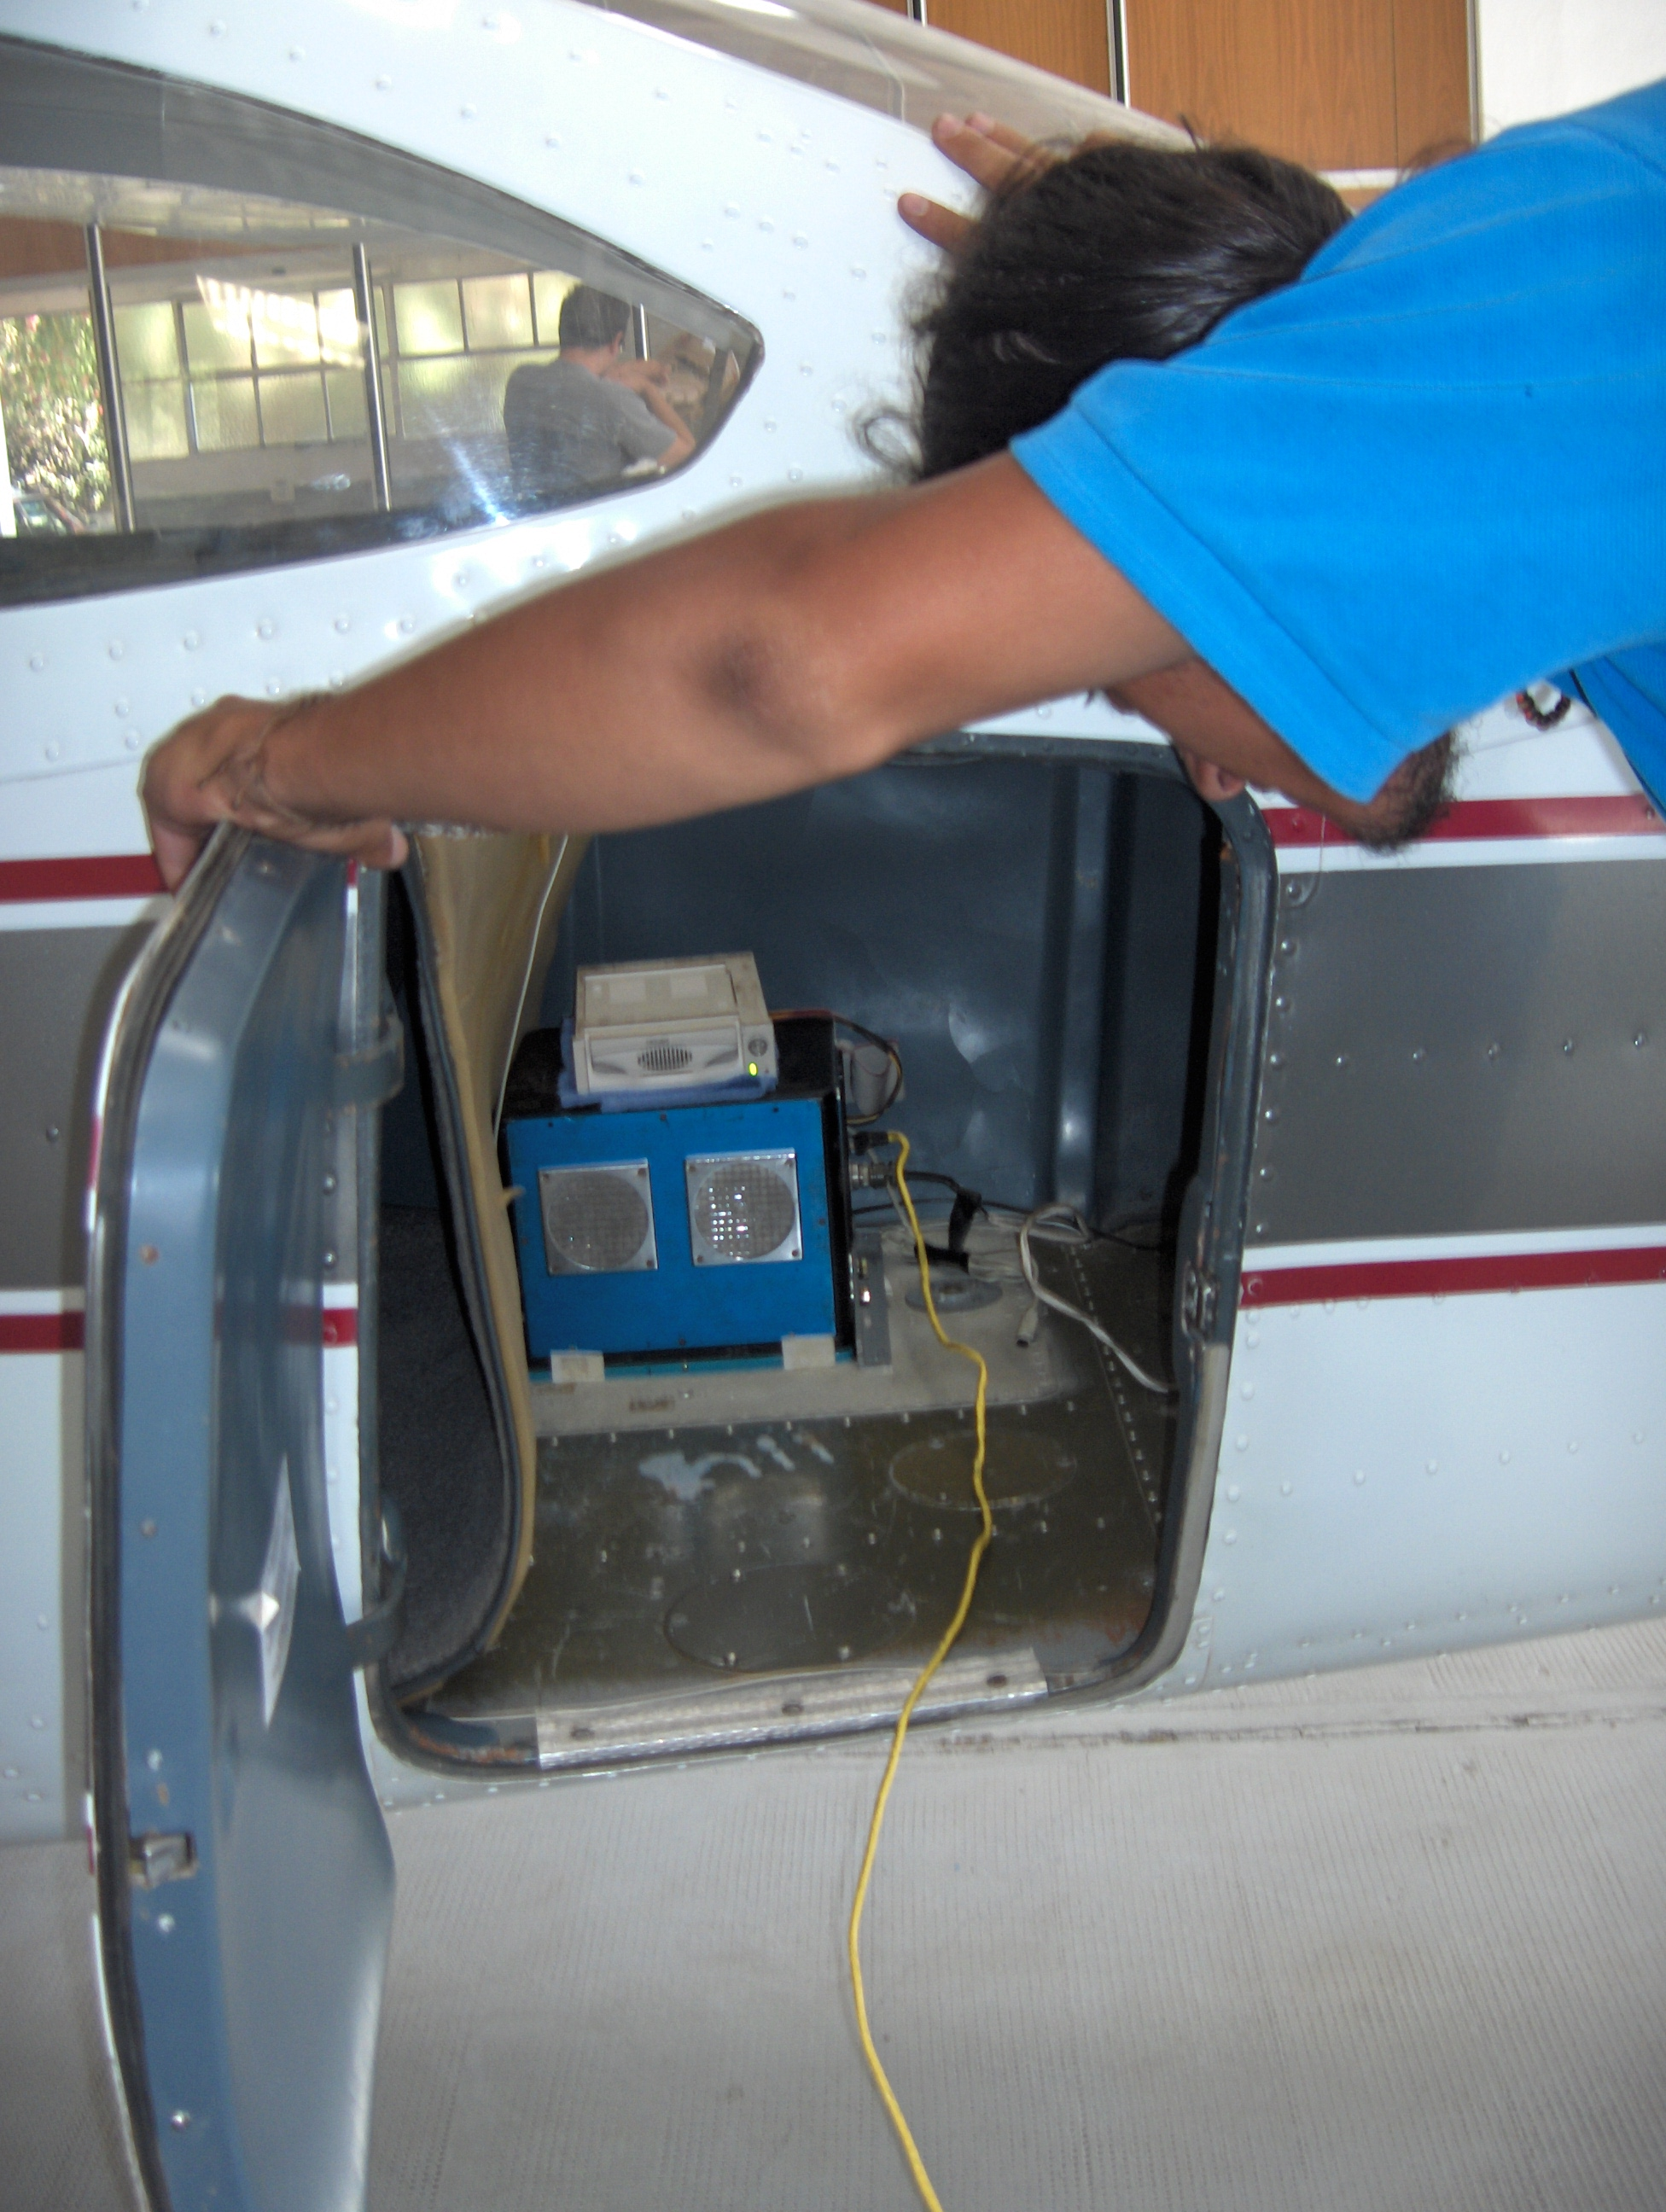
\includegraphics[width=0.9\textwidth]{IMGs/camarainta}
		\column{.5\textwidth}
		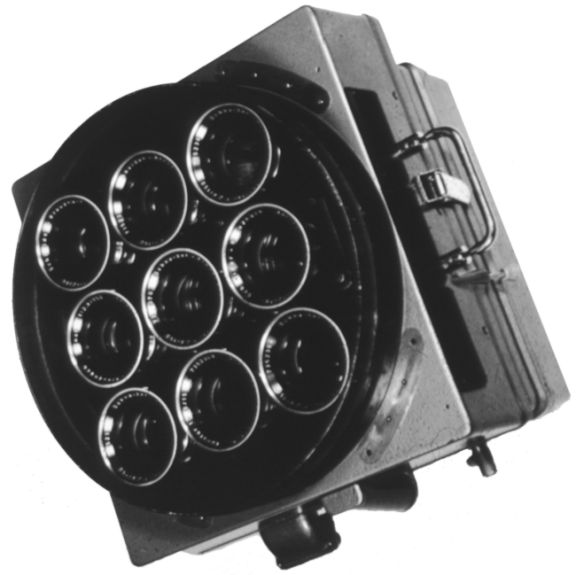
\includegraphics[width=0.6\textwidth]{IMGs/camara_multi}\\
		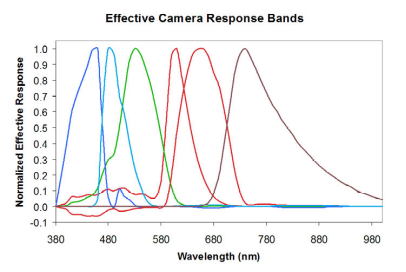
\includegraphics[width=0.75\textwidth]{IMGs/camara_multi2}
	\end{columns}
\end{frame}


\begin{frame}{Cámaras multiespectrales bajo-costo}
	\begin{columns}
		\column{.5\textwidth}
		\centering
		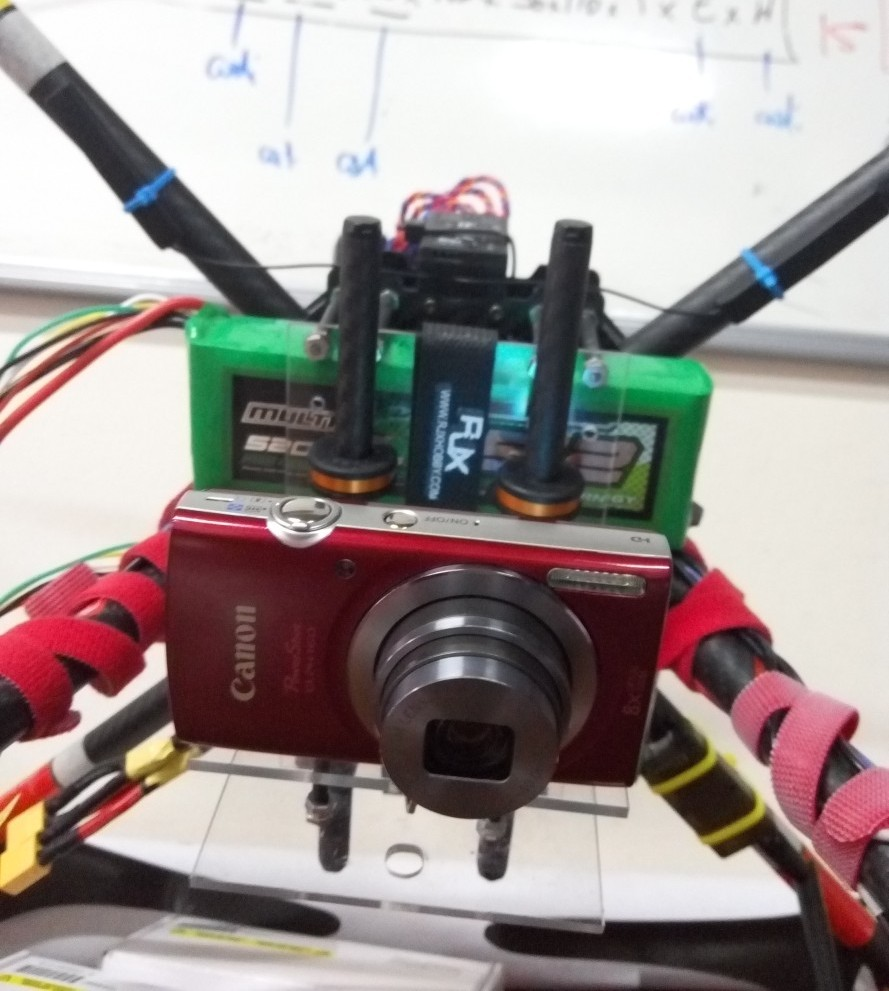
\includegraphics[width=0.6\textwidth]{IMGs/camara_UAV}\\
		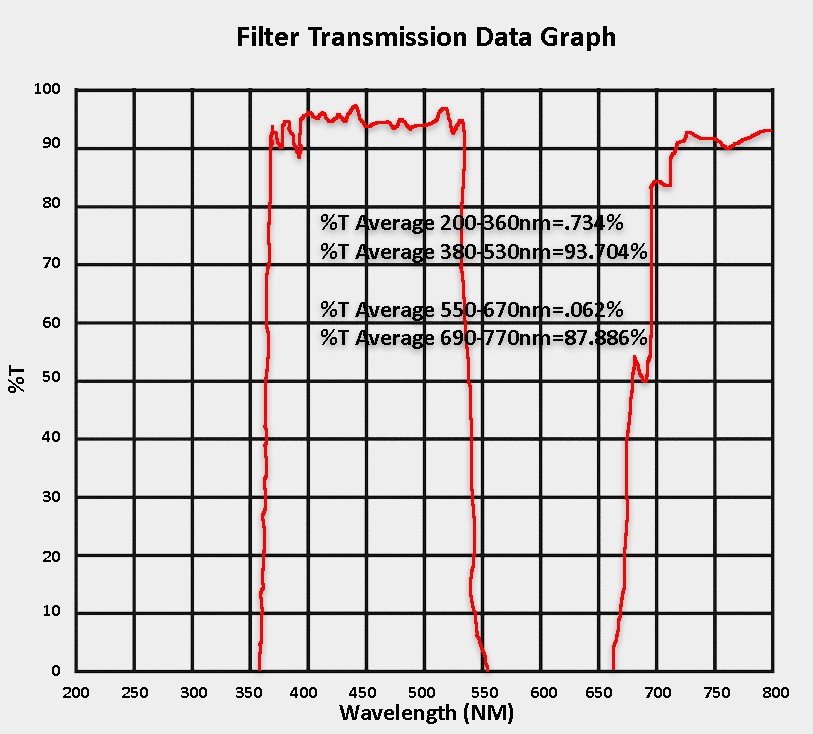
\includegraphics[width=0.7\textwidth]{IMGs/filtro_UAV}
		\column{.5\textwidth}
		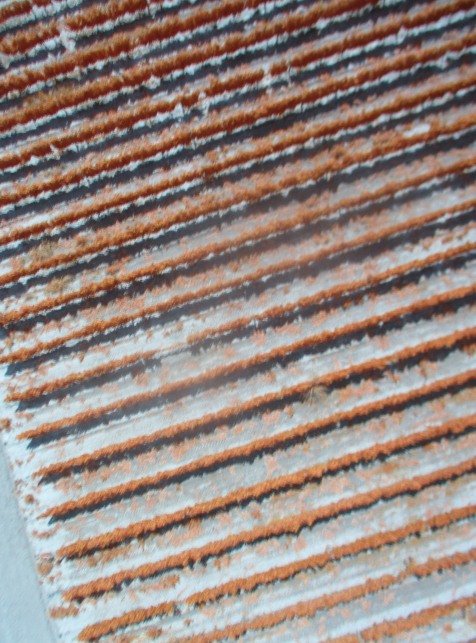
\includegraphics[width=0.85\textwidth]{IMGs/ngb}
	\end{columns}
\end{frame}

\begin{frame}{Resolución Temporal}
	\begin{itemize}
		\item Desarrollo de lo cultivos
		\item Fenómenos de corta duración (incendios, inundaciones)
		\item Dispersión de una enfermedad en un bosque
		\item Presencia de nubes
	\end{itemize}
\end{frame}

\begin{frame}{Resolución Angular}
	\begin{columns}
		\column{.5\textwidth}
		\centering
		\includegraphics<1->[width=0.6\textwidth]{IMGs/spot2}\\
		\includegraphics<2->[width=0.7\textwidth]{IMGs/spot1}
		\column{.5\textwidth}
		\includegraphics<3->[width=0.85\textwidth]{IMGs/spot3}
	\end{columns}
\end{frame}

\begin{frame}{Características orbitales}
	\begin{columns}
		\column{.5\textwidth}
		\begin{itemize}
			\item Elementos de la órbita.
			\item Area abarcada.
			\item Frecuencia de adquisición.
			\item Sensores disponibles.
		\end{itemize}
		\column{.5\textwidth}
		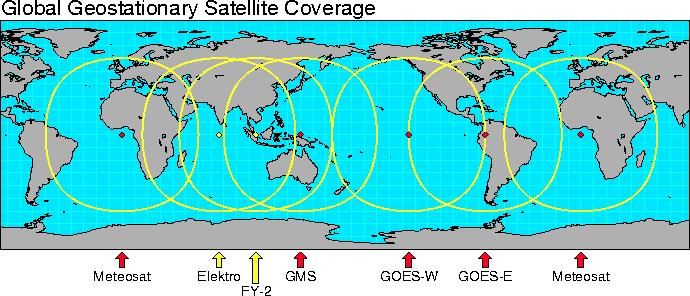
\includegraphics[width=0.85\textwidth]{IMGs/geoestat}\\
		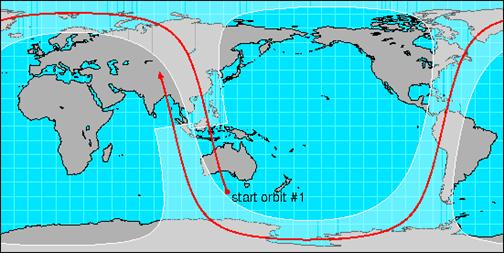
\includegraphics[width=0.85\textwidth]{IMGs/polar1}\\
		\includegraphics<2>[width=0.85\textwidth]{IMGs/polar2}
	\end{columns}
\end{frame}



\section{Radares}

\section{Acceso a los datos}

\end{document}

